\chapter{Análisis de alternativas}

\section{Arquitectura}

Se ha escogido una arquitectura de datos procesado de datos en tiempo real frente a una de procesado en lotes puesto que se necesita una latencia baja de procesado. Si se necesitara en un futuro un procesado por lotes, las arquitecturas de procesado en tiempo real puede hacer un procesado por lotes. La arquitectura planteada está basada en la arquitectura Kappa pero tiene ciertas variaciones en la manera en que guarda los archivos procesados.

En la Figura \ref{fig:arquitectura} podemos ver la arquitectura resultante. El dispositivo Android y Kafka compondrían el módulo de extracción, Logstash y Kafka Streams el módulo de transformación y Elastic Search, Kibana y JIRA el módulo de carga.

\subsubsection{Extracción}

Para la recolección y el envío de eventos en el dispositivo ubicuo se ha utilizado dos librerías, una recoge y envía crashlogs y otra recoge y envía logs. Se podría haber programado una librería propia que hiciese lo que estas dos, pero pareció mejor opción por la duración del proyecto el utilizar librerías que ya están testeadas y se saben que funcionan. 

Para garantizar que la extracción fuese escalable, en vez de enviar los eventos directamente hacia el sistema de ingesta de datos, se decidió colocar una REST API que hiciese de punto común a todos los dispositivos ubicuos, para el caso del proyecto tan solo son dispositivos Android, pero de esta manera se ofrece un punto de entrada al sistema a la gran mayoría de dispositivos ubicuos.

Antes de pasar al sistema de transformación, se decidió colocar un buffer de datos, Apache Kafka actúa como buffer de los datos enviados por los dispositivos ubicuos. Se podría no haber colocado y enviar directamente los datos al sistema de transformación, pero se ha colocado puesto que Kafka puede soportar picos elevados de eventos, es decir, es resiliente, de esta manera si hay un pico elevado de eventos el sistema de procesado no caería puesto que Kafka los retiene y el sistema de procesado los va consumiendo a su ritmo. Otra de las causas de utilizar Kafka, es para no perder los datos si por algún casual el sistema de procesado cayera. Si el sistema de procesado cayera, Kafka almacenaría los datos hasta que el sistema de procesado estuviera otra vez arriba y pudiera consumir dichos datos.

\subsubsection{Transformación}

Para la transformación de eventos, se ha utilizado por un lado Logstash y por otro Kafka Streams.

Logstash se ha utilizado ya que facilita mucho el procesado de los eventos y porque se integra excelentemente con Elastic Search. Alternativas al procesado de eventos que se integrasen tan bien no existían muchas.

Kakfa Streams se ha utilizado para hacer un procesado más inteligente de los datos cuando se requiera, puesto que Logstash nos ofrece un enriquecimiento de los datos más que un procesado inteligente. Se ha escogido de entre sus similares porque se integra a la perfección con Apache Kafka, ejecuta un Stream Processing real y porque el modo que tiene de desplegarse es rápido y fácil, no requiere de un clúster muy extenso para trabajar.

\subsection{Carga} 
Para la carga no habían alternativas puesto que hay que integrarse con Elastic Search y con JIRA. Otro sistema interesante para la motorización hubiese sido Nagios, pero tanto Elastic Search como JIRA cumplen sus propósito.

\begin{figure}
	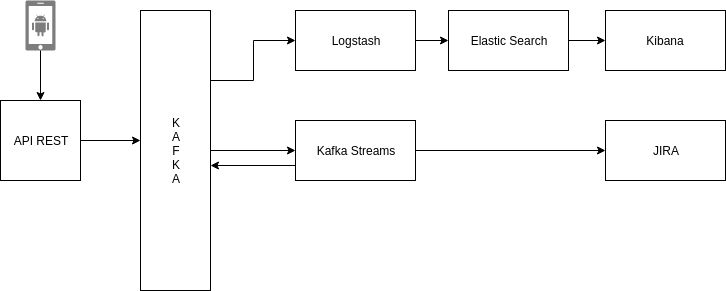
\includegraphics[width=\linewidth]{Arquitectura.png}
	\caption{Arquitectura resultante}
	\label{fig:arquitectura}
\end{figure}